\documentclass[11pt]{article}

\usepackage{sectsty}
\usepackage{graphicx}
\usepackage[T1]{fontenc}
\usepackage{multicol}
\usepackage{hyperref}
\usepackage{float}
% Margins
\topmargin=-0.5in
\evensidemargin=0in
\oddsidemargin=0in
\textwidth=6.5in
\textheight=9.0in
\headsep=0.25in

\title{ Analiza modelów regresji do przewidywania liczby ludności w Polsce}
\author{ Krzysztof Kulka
        \\ 272667@student.pwr.edu.pl \\ MSiD Lab Wtorek 9.15 NP }
\date{\today}

\renewcommand{\contentsname}{Spis treści}

\begin{document}
\maketitle	
\pagebreak

% Optional TOC
\tableofcontents
 \pagebreak

%--Paper--

\section{Wstęp}
Problemem projektu jest analiza możliwości modelów regresji liniowej do przewidywania liczby ludności w Polsce. W tym celu wykorzystane zostaną dane historyczne dotyczące demografi, oraz innych czynników wpływających na liczebność populacji.
Przedstawiona analiza ma na celu rozstrzygnięcie czy model regresji liniowej jest odpowiedni do przewidywania liczby ludności w Polsce, oraz jakie modele sprawdzają się do tego najlepiej.
Analizie zostaną poddane następujące czynniki:
\begin{itemize}
\item Historyczna liczba ludności
\item Imigracja do kraju
\item Wskaźnik dzietności
\item Oczekiwana długość życia
\item Urbanizacja
\item Wskaźnik zmiany populacji na przestrzeni ostatnich 5 lat
\end{itemize}
Zbadane zaś zostaną następujące modele regresji:
\begin{itemize}
\item Regresja liniowa
\item Regresja typu Ridge
\item Regresja Decisions Trees
\item Regresja Random Forest
\item Regresja Lasso
\end{itemize}
\section{Zbiór danych i jego analiza}
\subsection*{Opis zbioru danych}
Zbiór danych zawiera informacje na temat historycznej liczby ludności, imigracji do kraju, wskazniku dzietnosci, oczekiwanej długości życia w momencie urodzenia na przestrzeni lat 1960-2023.
Dane zostały pobrane z serwisu internetowego World Bank\cite{wbd} Dane dotyczą około 260 krajów. 
Dodatkowo informacje na temat urbanizacji
zostały pobrane z serwisu internetowego Zintegrowana Platforma Edukacyjna Ministerstwa Edukacji Narodowej\cite{zpe}, a wskaźnik zmiany populacji na przestrzeni ostatnich 5 lat został obliczony na podstawie danych historycznych.
\subsection*{Obróbka danych}
Najważniejszym krokiem w obróbce danych było wyizolowanie danych dotyczących Polski, oraz usunięcie kolumn, które nie były istotne dla analizy.
Dodatkowo, z racji tego że dane dotyczące imigracji rejestrowane co pięć lat, skorzystano z interpolacji liniowej, aby uzupełnić brakujące dane.
W późniejszym etapie, dane zostały obcięte do roku 2019, z powodu pandemii COVID-19, która znacząco wpłynęła na liczebność populacji i dane dotyczące demografii.
\subsection*{Analiza danych}
Do analizy eksploracyjnej danych wykorzystano bibliotekę pandas-profiling\cite{pp}
\subsection*{Populacja w Polsce}
\begin{figure}[H]
        \centering
        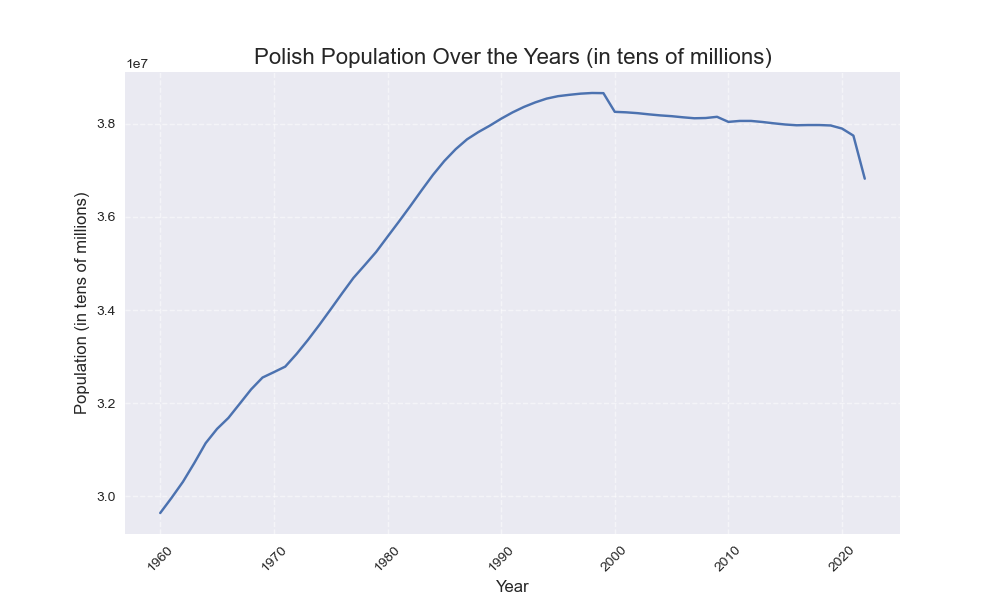
\includegraphics[width=0.8\textwidth]{polish_population_over_the_years.png}
        \caption{Wizualizacja liczby ludności w Polsce na przestrzeni lat}
\end{figure}
\begin{figure}[H]
        \centering
        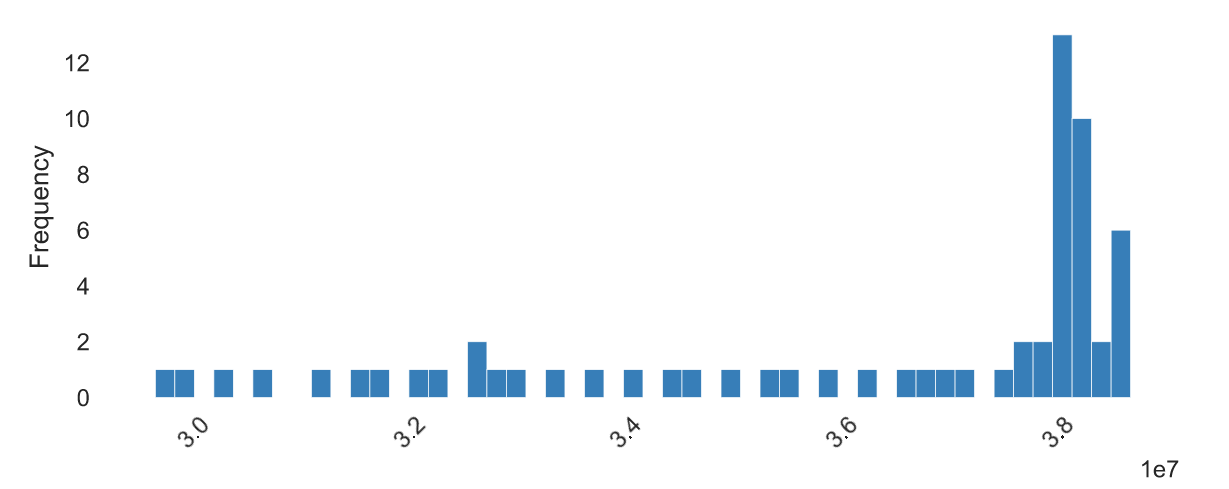
\includegraphics[width=0.8\textwidth]{images/histogram_populacja.png}
        \caption{Histogram liczby ludności w Polsce}
\end{figure}
\begin{table}[H]
        \centering
        \begin{tabular}{|l|l|l|}
        \hline
        Minimum & Maximum & Mediana \\ \hline
        29637450 & 38663481 & 37899070 \\ \hline
        \end{tabular}
        \caption{Statystyki liczby ludności w Polsce}
        \end{table}
\subsection*{Imigracja do Polski}
\begin{figure}[H]
        \centering
        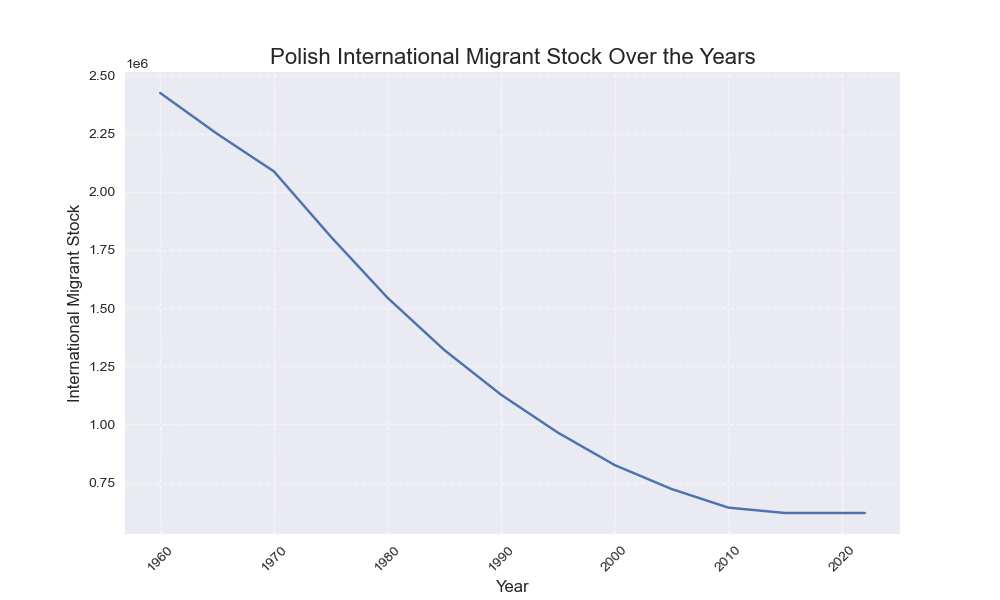
\includegraphics[width=0.8\textwidth]{polish_int_migrant_stock_over_the_years.png}
        \caption{Wizualizacja imigracji do Polski na przestrzeni lat}
\end{figure}
\begin{figure}[H]
        \centering
        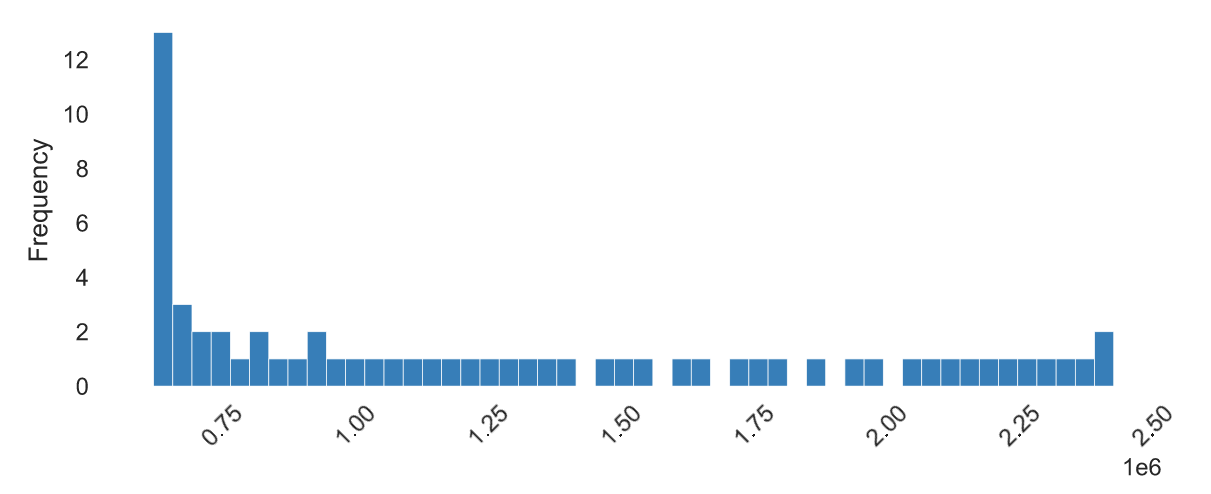
\includegraphics[width=0.8\textwidth]{images/histogram_imigracja.png}
        \caption{Histogram imigracji do Polski na przestrzeni lat}
\end{figure}
\begin{table}[H]
        \centering
        \begin{tabular}{|l|l|l|}
        \hline
        Minimum & Maximum & Mediana \\ \hline
        0 & 0 & 0 \\ \hline
        \end{tabular}
        \caption{Statystyki imigracji do Polski}
        \end{table}
\subsection*{Współczynnik dzietności}
\begin{figure}[H]
        \centering
        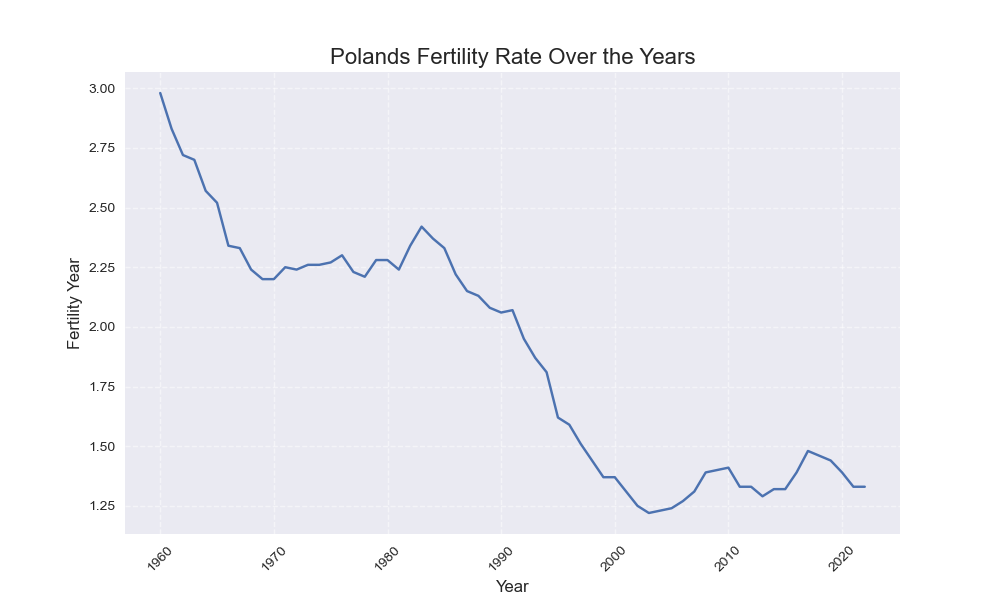
\includegraphics[width=0.8\textwidth]{polish_fertility_rate.png}
        \caption{Wizualizacja współczynnika dzietności Polski na przestrzeni lat}
\end{figure}
\begin{figure}[H]
        \centering
        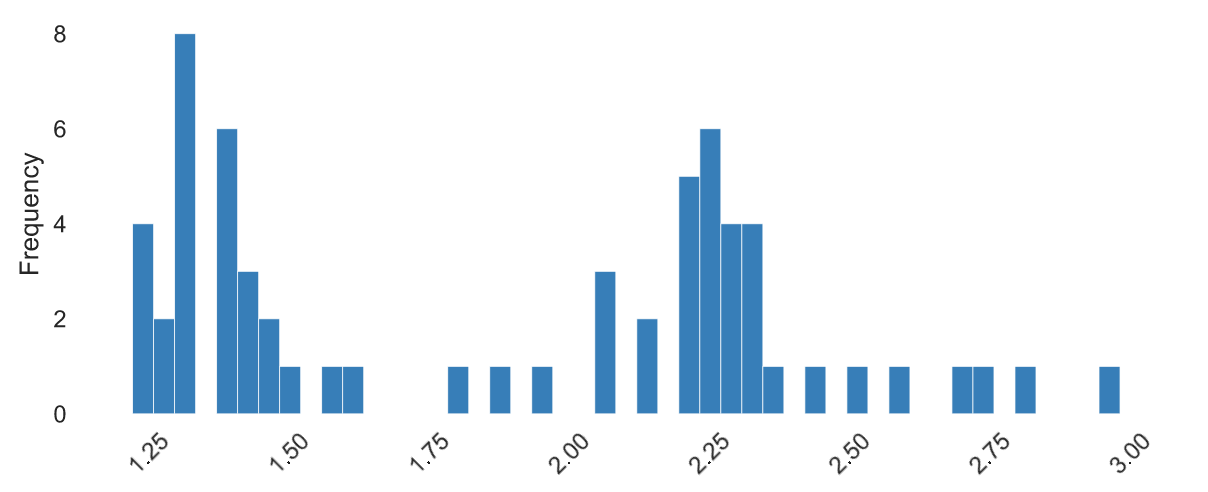
\includegraphics[width=0.8\textwidth]{images/histogram_dzietnosc.png}
        \caption{Histogram współczynnika dzietności na przestrzeni lat}
\end{figure}
\begin{table}[H]
        \centering
        \begin{tabular}{|l|l|l|}
        \hline
        Minimum & Maximum & Mediana \\ \hline
        1.4 & 1.6 & 1.5 \\ \hline
        \end{tabular}
        \caption{Statystyki współczynnika dzietności}
        \end{table}
\subsection*{Oczekiwana długość życia}
\begin{figure}[H]
        \centering
        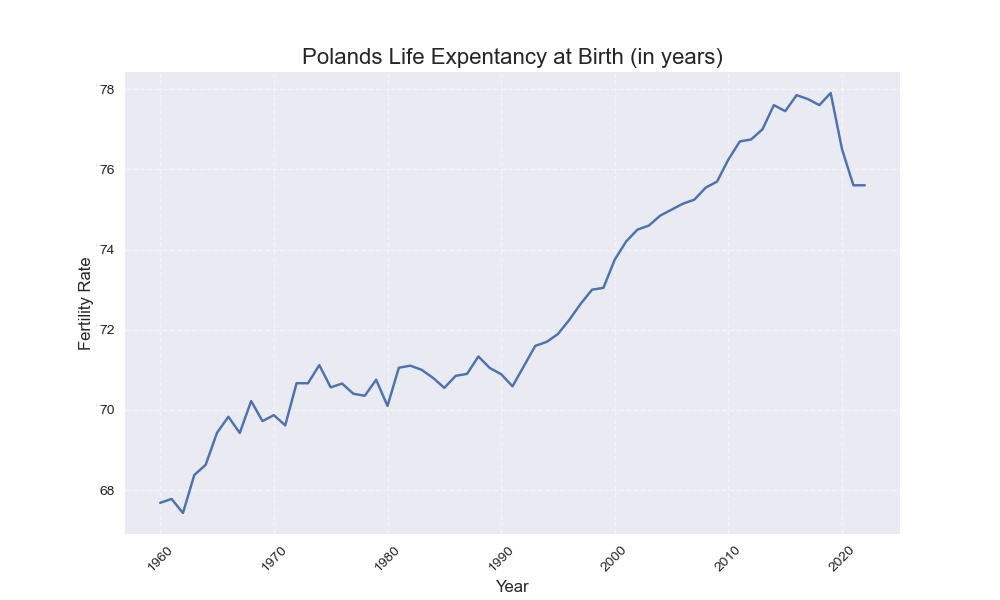
\includegraphics[width=0.8\textwidth]{polish_life_expentancy.png}
        \caption{Wizualizacja oczekiwanej długości życia na przestrzeni lat}
\end{figure}
\begin{figure}[H]
        \centering
        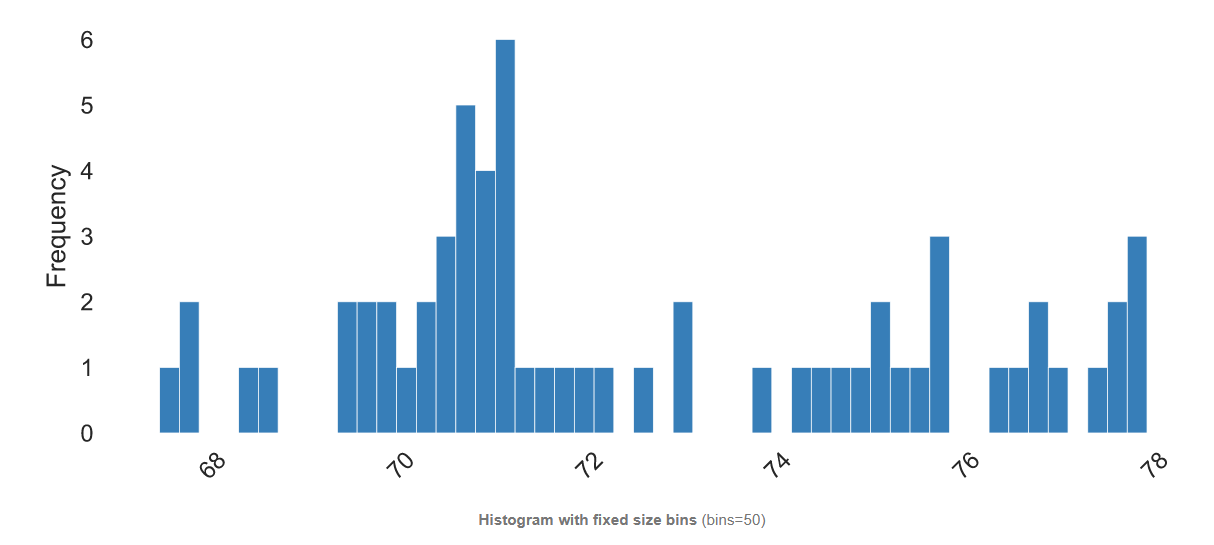
\includegraphics[width=0.8\textwidth]{images/histogram_dl_zycia.png}
        \caption{Histogram oczekiwanej długości życia na przestrzeni lat}
\end{figure}
\begin{table}[H]
        \centering
        \begin{tabular}{|l|l|l|}
        \hline
        Minimum & Maximum & Mediana \\ \hline
        70.0 & 80.0 & 75.0 \\ \hline
        \end{tabular}
        \caption{Statystyki oczekiwanej długości życia}
        \end{table}
\subsection*{Urbanizacja}
\begin{figure}[H]
        \centering
        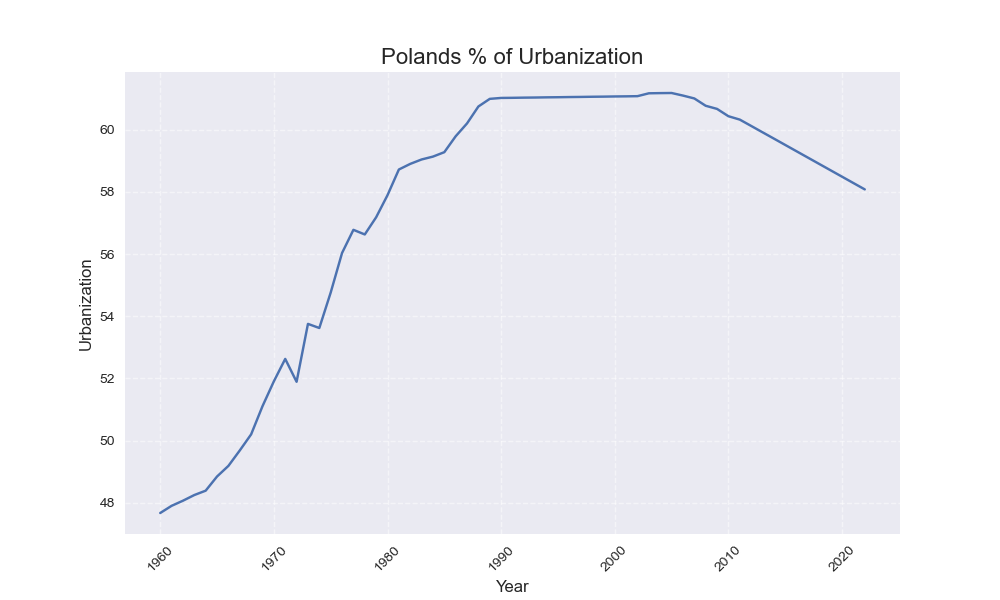
\includegraphics[width=0.8\textwidth]{polish_urbanization.png}
        \caption{Wizualizacja urbanizacji na przestrzeni lat}
\end{figure}
\begin{figure}[H]
        \centering
        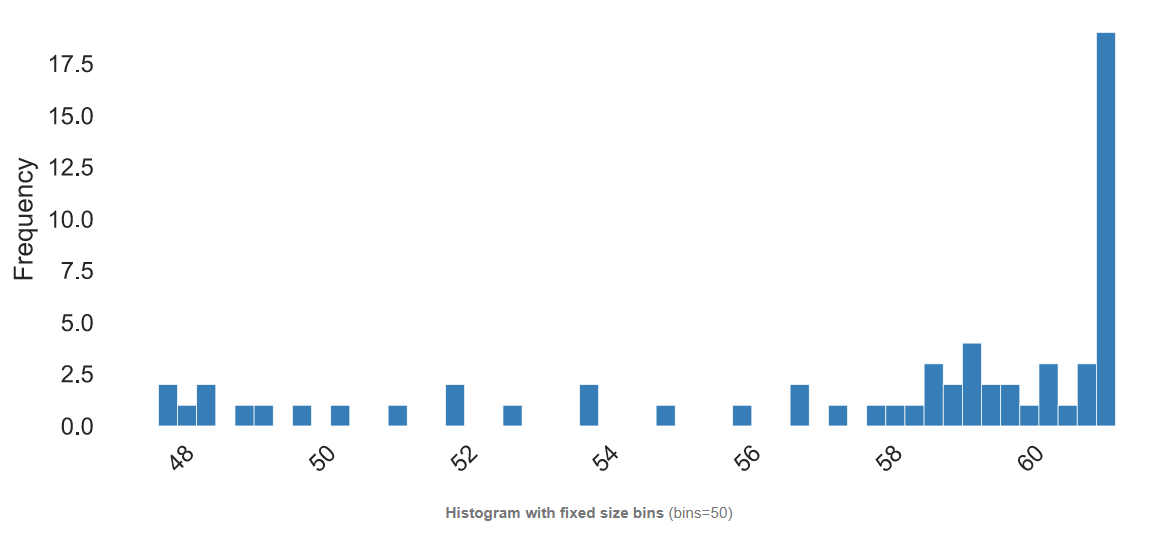
\includegraphics[width=0.8\textwidth]{images/histogram_urbanizacja.png}
        \caption{Wizualizacja urbanizacji na przestrzeni lat}
\end{figure}
\begin{table}[H]
        \centering
        \begin{tabular}{|l|l|l|}
        \hline
        Minimum & Maximum & Mediana \\ \hline
        0.0 & 0.0 & 0.0 \\ \hline
        \end{tabular}
        \caption{Statystyki urbanizacji}
        \end{table}
\subsection*{Wskaźnik zmiany populacji}
\begin{figure}[H]
        \centering
        %\includegraphics[width=0.8\textwidth]{polish_population_growth.png}
        \caption{Wizualizacja wskaźnika zmiany populacji na przestrzeni lat}
\end{figure}
\begin{figure}[H]
        \centering
        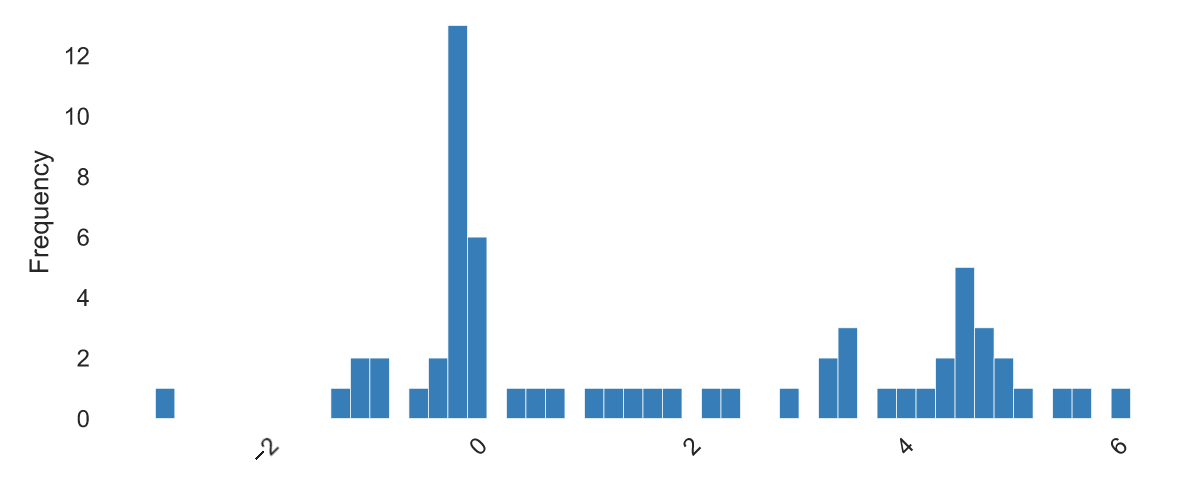
\includegraphics[width=0.8\textwidth]{images/histogram_zmiana_populacji.png}
        \caption{Histogram zmiany polskiej populacji na przestrzeni ostatnich 5 lat}
\end{figure}
\begin{table}[H]
        \centering
        \begin{tabular}{|l|l|l|}
        \hline
        Minimum & Maximum & Mediana \\ \hline
        -0.0001 & 0.0001 & 0.0 \\ \hline
        \end{tabular}
        \caption{Statystyki wskaźnika zmiany populacji}
        \end{table}
\bibliographystyle{plain}
\bibliography{bibliografia}
\end{document}
